\documentclass[12pt,a4paper]{article}

\setlength{\headheight}{15.08075pt}
\addtolength{\topmargin}{-2.84344pt}

% Suporte para a língua portuguesa
\usepackage[utf8]{inputenc}
\usepackage[T1]{fontenc}
\usepackage[brazil]{babel}

% Melhorias de tipografia
\usepackage{microtype}

% Cores personalizadas
\usepackage{xcolor}
\definecolor{darkblue}{RGB}{25,25,112}

% Para cabeçalhos bonitos
\usepackage{fancyhdr}

% Controlar layout da página
\usepackage{geometry}
\geometry{
    a4paper,
    total={170mm,257mm},
    left=20mm,
    top=20mm,
}

% Para inserção e manipulação de imagens
\usepackage{graphicx}
\graphicspath{{imagens/}} % Define o diretório padrão das imagens
\usepackage{float} % Para melhor controle de posicionamento

% Para títulos de seções coloridos e personalizados
\usepackage{titlesec}
\titleformat{\section}
{\color{darkblue}\normalfont\Large\bfseries}
{\color{darkblue}\thesection}{1em}{}

\titleformat{\subsection}
{\color{darkblue}\normalfont\large\bfseries}
{\color{darkblue}\thesubsection}{1em}{}

% Para links e referências
\usepackage{hyperref}
\hypersetup{
    colorlinks=true,
    linkcolor=darkblue,
    filecolor=magenta,      
    urlcolor=cyan,
    citecolor=darkblue,
}
% Permite quebras de linha em URLs em qualquer lugar, melhorando a quebra de linhas longas
\usepackage{xurl}

% Para alguns símbolos adicionais
\usepackage{fontawesome}

% Para caixas coloridas
\usepackage[most]{tcolorbox}

% para formatação de células de tabelas
\usepackage{array} 

\usepackage{multicol} % para multiplas colunas

\usepackage{caption} % para legendas de figura

\tcbuselibrary{skins} % Usar skins do tcolorbox

% Comandos
\newcommand{\DonwloadUrl}{\url{https://www.intel.com.br/content/www/br/pt/products/details/fpga/development-tools/quartus-prime/resource.html}}
\newcommand{\Version}{18.1}

% \newcommand{\Attention}[1]{
%     \begin{tcolorbox}[colback=red!5!white,colframe=red!75!black]
%     \begin{center}
%     \faExclamationTriangle{}\\#1
%     \end{center}
%     \end{tcolorbox}
% }

\newcommand{\Attention}[1]{
    \begin{tcolorbox}[colback=red!5!white, colframe=red!75!black]
        \noindent
        \begin{minipage}[c]{1cm}% Largura para a imagem
            
\includegraphics[width=\linewidth]{figs/attention.png}
        \end{minipage}%
        \hfill% Espaço entre a imagem e o texto
        \begin{minipage}[c]{\dimexpr\linewidth-1cm-2mm}% Largura para o texto, ajustando o espaço
            \begin{center}
                #1    
            \end{center}            
        \end{minipage}
    \end{tcolorbox}
}


\pagestyle{fancy}
\fancyhf{}
\rhead{\textbf{Lógica Reconfigurável/Tutorial 1}}
\lhead{\textbf{\leftmark}}
\cfoot{\thepage}

\title{\textbf{Criando e Simulando Circuitos Digitais no Quartus}}
\author{Prof. Felipe W. D. Pfrimer}
\date{\today}

\begin{document}

\maketitle
\newpage
\tableofcontents
\newpage

\section{Introdução}

O IntelFPGA Quartus Prime representa uma plataforma abrangente de desenvolvimento para Dispositivos Lógicos Programáveis (PLDs), oferecida pela IntelFPGA. Este Ambiente de Desenvolvimento Integrado (IDE) capacita os desenvolvedores na criação, análise, e síntese de sistemas digitais, empregando Linguagens de Descrição de Hardware (HDLs) ou diagramas esquemáticos. A versão Lite do Quartus Prime, especificamente a \Version, está disponível gratuitamente e pode ser obtida diretamente através do site da Intel, usando a macro LaTeX para URLs como segue: \DonwloadUrl.%\url{https://www.intel.com.br/content/www/br/pt/products/details/fpga/development-tools/quartus-prime/resource.html}.

Este tutorial é direcionado a fornecer ao leitor uma introdução prática ao desenvolvimento e simulação de sistemas digitais utilizando diagramas esquemáticos no Quartus Prime Lite \Version. Embora nosso foco esteja na versão \Version, é importante notar que os princípios e procedimentos aqui descritos podem ser aplicáveis a outras versões do software, podendo haver pequenas alteração dependendo da versão utilizada.


\section{Objetivo do Tutorial}

O objetivo principal deste tutorial é guiar o leitor através do processo de simulação funcional de um somador \textit{carry ripple} de 4 bits, o qual será projetado utilizando diagramas de blocos. Através deste guia, você aprenderá como configurar, implementar e simular um circuito digital básico dentro do ambiente de desenvolvimento do Quartus Prime Lite \Version, focando especificamente na versão funcional de simulação.

\section{Conceitos importantes}

Essa seção trata de alguns conceitos importantes para o entendimento deste tutorial.

\subsection{O que é Simulação Funcional?}

A simulação funcional é uma técnica fundamental no design de circuitos digitais, permitindo aos designers verificar e analisar o comportamento de um circuito sem a necessidade de construí-lo fisicamente. Este método de simulação envolve a execução de um modelo de software do circuito para testar suas funções sob várias condições de entrada, assegurando que ele atenda às especificações desejadas antes de prosseguir para a etapa de implementação física.

Na simulação funcional, o foco está em validar a lógica e as operações do circuito, sem levar em conta as características físicas dos componentes, como atrasos de tempo ou consumo de energia. Isso permite uma verificação rápida e eficiente do design em nível lógico, facilitando a detecção e correção de erros em estágios iniciais do desenvolvimento do projeto.

Ao concluir este tutorial, você terá adquirido conhecimentos práticos sobre como realizar simulações funcionais de circuitos digitais, usando o exemplo prático de um somador de 4 bits para ilustrar os conceitos e procedimentos envolvidos. Este conhecimento será valioso para futuros projetos de design de circuitos, permitindo uma abordagem mais eficaz e eficiente na verificação de designs antes da implementação.

\subsection{O Quartus Prime}

O Quartus Prime \cite{QuartusPrimeUserGuide} é uma IDE (\textit{Integrated Development Environment}) desenvolvida pela Intel, anteriormente pela Altera, para o design, simulação, programação e depuração de sistemas digitais integrados, incluindo FPGAs (\textit{Field-Programmable Gate Arrays}), CPLDs (\textit{Complex Programmable Logic Devices}) e SoCs (\textit{Systems on Chips}). Como uma IDE, o Quartus Prime integra ferramentas e funcionalidades ao desenvolvimento de hardware, auxiliando engenheiros e projetistas na criação de sistemas eletrônicos.

Uma IDE é um software que oferece ferramentas para programadores e desenvolvedores, como edição de código, compilação, depuração e, em alguns casos, simulação. A principal função de uma IDE é proporcionar um ambiente que otimize a produtividade, reduzindo a necessidade de alternar entre diferentes aplicações durante o desenvolvimento de software ou hardware. Uma IDE serve como uma plataforma onde desenvolvimento, testes e depuração ocorrem de forma integrada.

No contexto do Quartus Prime, a IDE se especializa no design e implementação de componentes eletrônicos programáveis. Permite aos usuários elaborar esquemáticos, escrever e testar códigos em linguagens de descrição de hardware como VHDL e Verilog, e simular o comportamento de circuitos digitais antes da implementação física. Adicionalmente, o Quartus Prime simplifica a programação dos dispositivos com os designs desenvolvidos, sendo uma ferramenta importante na engenharia eletrônica para o desenvolvimento de sistemas digitais.

\section{Somadores \textit{carry ripple}}

Um somador digital é um circuito que executa a soma de dois números binários e considera um \textit{carry-in} (um bit adicional de uma soma anterior). Este circuito é utilizado na construção de sistemas de computação e processamento digital, habilitando operações aritméticas básicas\cite{YouTube2020luiz,Tocci2007SistemasDigitais}.

Um somador \textit{carry ripple} é construído pela concatenação de somadores completos de 1 bit, onde cada somador processa dois bits e um \textit{carry-in}, resultando em um bit de soma e um \textit{carry-out}. A principal limitação dessa abordagem reside na velocidade de operação. Especificamente, o tempo de cálculo de uma soma aumenta proporcionalmente ao número de bits envolvidos, devido à necessidade de esperar a propagação do \textit{carry-out} de um somador para o \textit{carry-in} do somador subsequente \cite{YouTube2021descomplica}.

Esta propagação sequencial do \textit{carry} implica que o bit de \textit{carry} precisa ``viajar'' por todos os somadores na cadeia, um após o outro, antes que a soma total possa ser completada. Assim, para somas de números com muitos bits, o atraso total introduzido pela propagação do \textit{carry} pode se tornar significativo, impactando negativamente o desempenho da operação de soma em aplicações que demandam alta velocidade e baixa latência. No entanto, devido a sua simplicidade, esse tipo de abordagem é ideal para os propósitos deste guia.

%Uma das formas de se construir um somador digital consiste na concatenação de circuitos somadores de 1 bit \cite{YouTube2021descomplica}, numa estrutura chamada somador \textit{carry ripple}. Um somador completo de 1 bit soma dois bits e um \textit{carry-in}, produzindo um bit de soma e um \textit{carry-out} (``vai um''). O \textit{carry-out} de um somador serve como \textit{carry-in} para o próximo, permitindo a soma correta de números maiores que 1.

Ao conectar quatro somadores completos em sequência, pode-se somar dois números de 4 bits. O primeiro somador recebe os bits menos significativos dos números a serem somados, junto com o \textit{carry-in} inicial (geralmente 0). O \textit{carry-out} deste somador é passado como \textit{carry-in} para o somador subsequente, até o último somador, cujo \textit{carry-out} representa o \textit{carry-out} final da operação de soma.

Esta metodologia não apenas simplifica o design, mas também permite escalabilidade, facilitando a expansão para somadores de maiores dimensões através do aumento do número de somadores completos concatenados. %No entanto, a desvantagem do somador \textit{carry ripple} (ou somador de propagação de carry) é a sua velocidade de operação, que pode ser relativamente lenta para somas de números grandes. Isso ocorre porque, em um somador carry ripple, o carry de cada bit somado precisa ser calculado e propagado para o próximo bit mais significativo antes que este possa ser somado corretamente. Em outras palavras, o bit de carry gerado em cada etapa de soma (cada bit) precisa "viajar" através de todos os somadores de bit individuais na cadeia, um após o outro.

\section{Instalação}

Essa seção do tutorial destina-se a auxiliar na instalação do Quartus Prime Lite \Version{} em sistemas operacionais Windows 10 ou 11. Caso já possua o Quartus instalado, vá para a seção~\ref{sec:proj}.

\subsection{Download do Software}

\begin{enumerate}
    \item Acesse a página oficial de downloads da Intel para o Quartus Prime Lite \Version{} por meio do link: \DonwloadUrl;
    \item Na página, procure pela seção de downloads do \textbf{Quartus Prime Lite} Edition;
    
    \Attention{Certifique-se de escolher a versão Lite \Version.}

    \item Selecione a versão apropriada para Windows e clique no grande botão azul botão de download, na aba de \textit{Multiple Download}, para baixar todos os arquivos necessários;
    \item Aguarde baixar o arquivo de extensão .tar;
    % \item Enquanto o arquivo é baixado, hidrate-se ou tome um café 
\includegraphics[height=1em]{latte-art.png};
    \item Pode ser necessário criar uma conta Intel ou fazer login com uma conta existente para prosseguir com o download.
\end{enumerate}

\subsection{Instalação do Software}

\begin{enumerate}
    \item Uma vez concluído o download, localize o arquivo baixado e execute-o com um duplo clique;
    \item Se for exibida uma janela pedindo permissão para que o aplicativo faça alterações no seu dispositivo, clique em ``Sim'';
    \item Siga as instruções apresentadas pelo assistente de instalação. Aceite os termos de licença e selecione o diretório de instalação conforme desejado (de preferência, deixe o diretório proposto);
    \item Durante a instalação, você pode selecionar os componentes específicos do Quartus que deseja instalar (dispositivos). Para uma instalação padrão, é recomendável deixar as opções pré-selecionadas;
    
    \Attention{Tenha certeza de manter a família MAX10 e o modelsim IntelFPGA Edition ou Altera Edition. O modelsim padrão é um aplicativo que exige a compra de uma licença.}

    \item Após configurar suas preferências, prossiga com a instalação e aguarde até que o processo seja concluído. %Isso pode demorar bastante, recomenda-se café 
\includegraphics[height=1em]{latte-art.png}.
\end{enumerate}

\subsection{Inicialização do Programa}

\begin{enumerate}
    \item Após a conclusão da instalação, você pode iniciar o Quartus Prime Lite \Version{} através do menu Iniciar do Windows, procurando por "Quartus Prime Lite" ou através do atalho criado na área de trabalho, se disponível.
    \item Na primeira execução, pode ser necessário configurar algumas preferências iniciais ou realizar o registro do software, dependendo das exigências do programa.
    \item Com o Quartus Prime Lite aberto, você está agora pronto para começar a criar e simular seus projetos de sistemas digitais.
\end{enumerate}

Este guia deve ajudar você a instalar e iniciar o Quartus Prime Lite \Version{} em sua máquina Windows com facilidade. Para qualquer suporte adicional ou questões técnicas, referencie a documentação oficial do Quartus ou os fóruns de suporte da Intel.


\section{Criando um novo projeto}
\label{sec:proj}

A \autoref{fig:StartSc} ilustra a tela inicial do Quartus Prime Lite \Version.

\Attention{É crucial seguir os próximos passos exatamente como descritos e prestar atenção especial aos nomes dos arquivos mencionados. A precisão é essencial para o sucesso da configuração.}

\begin{figure}[htbp]
    \centering
    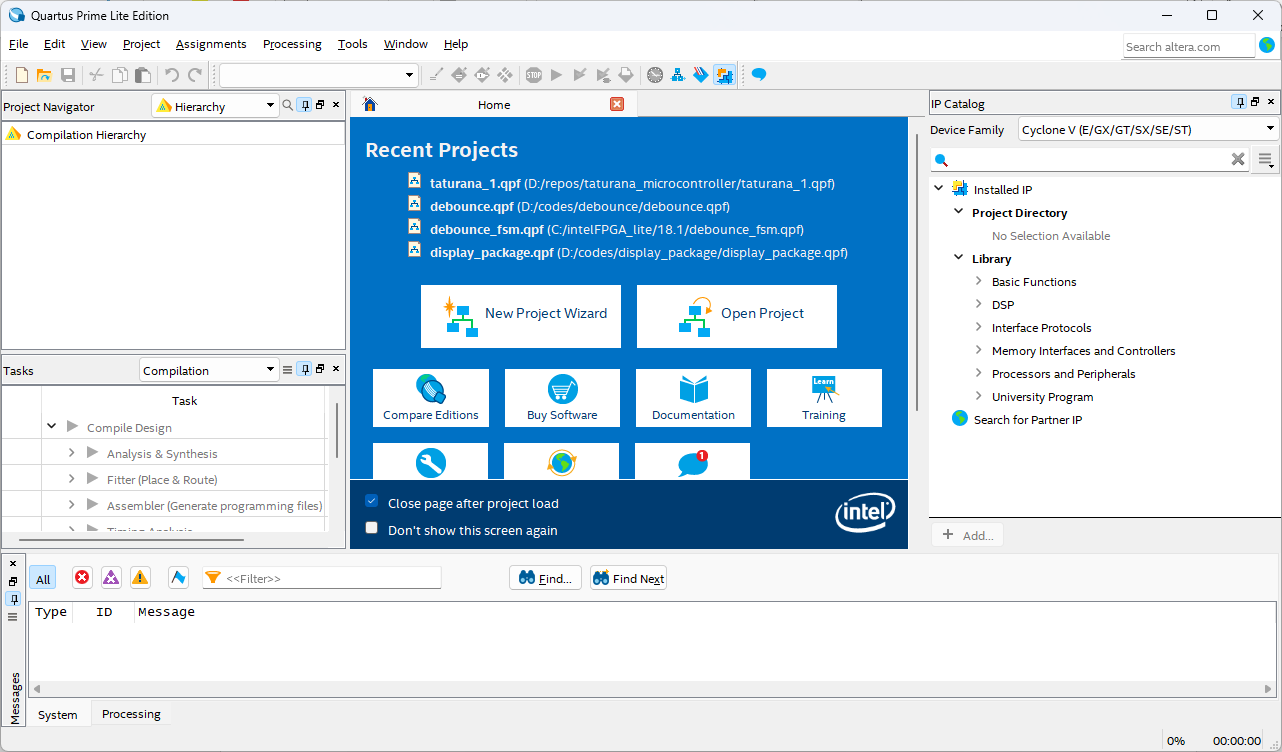
\includegraphics[width=\textwidth]{./figs/StartSc.png}
    \caption{Tela inicial do Quartus Prime Lite \Version.}
    \label{fig:StartSc}
\end{figure}

Um novo projeto pode ser criado clicando em \texttt{New Project Wizard} ou acessando o menu \texttt{File} $\rightarrow$ \texttt{New Project Wizard}. O \textit{Project Wizard} será aberto em uma nova janela para configurar o projeto, como ilustrado na Figura~\ref{fig:NewPj}. Nesta primeira tela, uma breve introdução sobre a criação de projetos será apresentada. Assim, basta clicar em \texttt{Next} e uma nova tela se abrirá, conforme mostrado na Figura~\ref{fig:Directory}, onde será possível escolher o diretório do projeto.

\begin{figure}[htbp!]
    \centering
    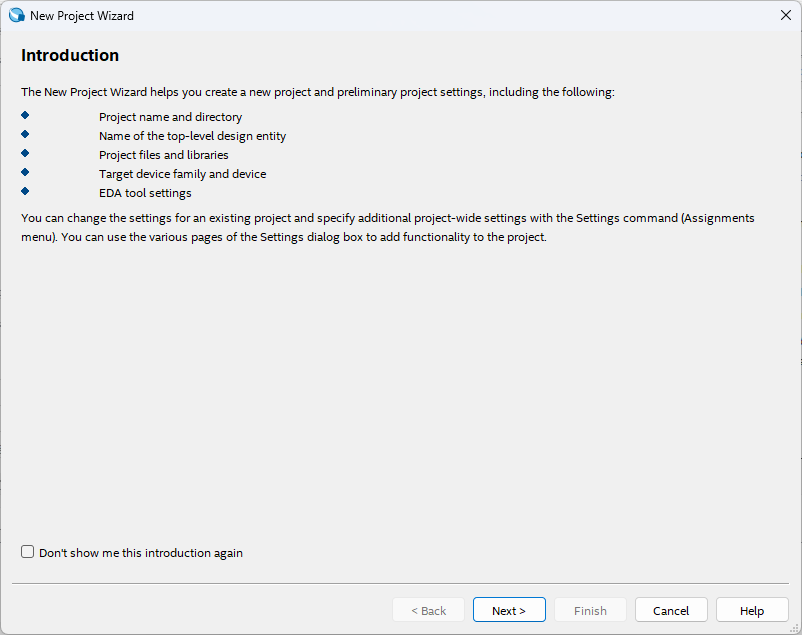
\includegraphics[width=0.8\textwidth]{./figs/NewPj.png}
    \caption{Tela inicial do \texttt{New Project Wizard}.}
    \label{fig:NewPj}
\end{figure}

\begin{figure}[htbp!]
    \centering
    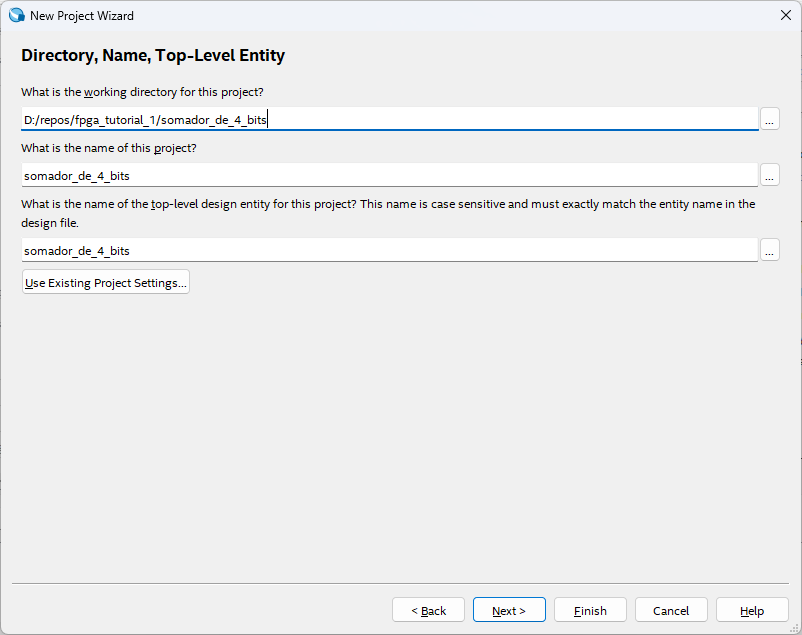
\includegraphics[width=0.8\textwidth]{./figs/Directory.png}
    \caption{Tela para escolha do diretório, nome do projeto e \textit{Top Lavel}.}
    \label{fig:Directory}
\end{figure}

Ao configurar um novo projeto no Quartus Prime Lite \Version, é essencial prestar atenção aos seguintes campos na tela de configuração do projeto:

\begin{enumerate}
    \item No primeiro campo, selecione o diretório que armazenará os arquivos do projeto. É necessário escolher um caminho de diretório (o caminho completo) livre de espaços e caracteres especiais da língua portuguesa, como cedilha (\texttt{\c{c}}) e vogais acentuadas. Para nosso exemplo, o diretório será nomeado como \texttt{somador\_de\_4\_bits}, já que o objetivo é criar um circuito somador.
    
    \item Na interface apresentada na Figura~\ref{fig:Directory}, insira o nome do projeto no segundo campo: \texttt{somador\_de\_4\_bits}. Observe que o terceiro campo é preenchido automaticamente com o mesmo nome do projeto. Este campo refere-se ao nome do arquivo principal do projeto (\textit{top-level design}). Embora seja possível modificar o nome no terceiro campo, evite iniciar o nome do arquivo principal com números, como em \texttt{4\_bit\_adder}. 
\end{enumerate}

Após ajustar esses detalhes, clique em \texttt{Finish}. Assim, um projeto vazio será criado. Dado que este exemplo foca em uma simulação funcional, a seleção de um dispositivo específico para programação não é exigida, algo que seria feito em telas de configuração posteriores; o programa automaticamente escolherá um dispositivo padrão. O próximo passo envolve a criação do primeiro arquivo esquemático do projeto.

\section{Primeiro esquemático}

Para este tutorial, vamos criar um somador \textit{carry ripple} de 4 bits. Contudo, a elaboração de tal somador requer a construção de um circuito \textbf{somador completo}, que será replicado quatro vezes no circuito final. Para mais informações sobre somadores digitais, consulte a referência \cite{Tocci2007SistemasDigitais}. 

O circuito de um somador completo, bem como sua tabela verdade, estão ilustrados na Figura~\ref{fig:somadorCompleto} e Tabela~\ref{table:full_adder_truth_table}, respectivamente. Observe que o circuito possui três entradas ($A$, $B$ e \textit{Carry in}) e duas saídas (\textit{Sum} e \textit{Carry out}). Além disso, é composto por cinco portas lógicas: duas \texttt{XOR}, duas \texttt{AND} e uma \texttt{OR}. Neste ponto, é interessante que o leitor tente deduzir o circuito lógico a partir da tabela verdade, utilizando métodos de simplificação de expressões booleanas, embora isso seja opcional.

\vspace{12pt}

\noindent % Remove a indentação
\begin{minipage}{0.45\textwidth}
    \centering
    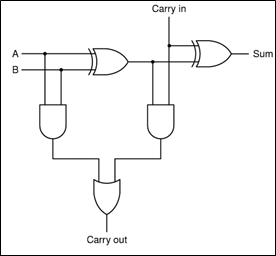
\includegraphics[width=0.9\textwidth]{./figs/FullAdder.png}
    \captionof{figure}{Circuito do somador completo.}
    \label{fig:somadorCompleto}
\end{minipage}\hfill % Espaçamento entre as minipages
\begin{minipage}{0.45\textwidth}
    \centering
    \begin{tabular}{ccc|cc}
    \hline
    \texttt{A} & \texttt{B} & \texttt{Carry\_in} & \texttt{Sum} & \texttt{Carry\_out} \\ \hline
    \texttt{0} & \texttt{0} & \texttt{0} & \texttt{0} & \texttt{0} \\
    \texttt{0} & \texttt{0} & \texttt{1} & \texttt{1} & \texttt{0} \\
    \texttt{0} & \texttt{1} & \texttt{0} & \texttt{1} & \texttt{0} \\
    \texttt{0} & \texttt{1} & \texttt{1} & \texttt{0} & \texttt{1} \\
    \texttt{1} & \texttt{0} & \texttt{0} & \texttt{1} & \texttt{0} \\
    \texttt{1} & \texttt{0} & \texttt{1} & \texttt{0} & \texttt{1} \\
    \texttt{1} & \texttt{1} & \texttt{0} & \texttt{0} & \texttt{1} \\
    \texttt{1} & \texttt{1} & \texttt{1} & \texttt{1} & \texttt{1} \\ \hline
    \end{tabular}
    \captionof{table}{Tabela verdade de um somador completo}
    \label{table:full_adder_truth_table}
\end{minipage}

\vspace{12pt}

Para a criação do esquemático do somador completo, clique em \texttt{File} $\rightarrow$ \texttt{New} e uma janela se abrirá com várias opções, conforme ilustrado na Figura~\ref{fig:file_type}. Escolha a opção \texttt{Block Diagram/Schematic File} e clique em \texttt{OK}. Um ambiente para edição de circuitos será aberto.

\newcolumntype{M}[1]{>{\centering\arraybackslash}m{#1}} % Coluna centralizada com largura fixa

\vspace{12pt}
\begin{minipage}{0.45\textwidth}
    \centering
    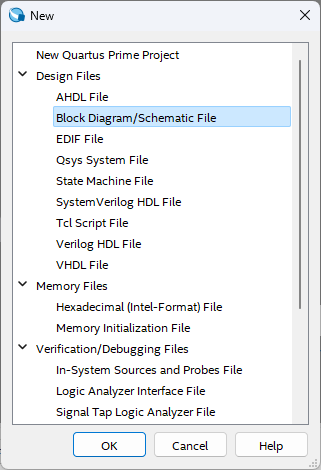
\includegraphics[width=\textwidth]{./figs/file_type.png}
    \captionof{figure}{Opções de novos arquivos.}
    \label{fig:file_type}
\end{minipage}\hfill
\begin{minipage}{0.45\textwidth}
    \centering    
    \begin{tabular}{M{1cm} M{5.5cm}}
    \hline
    \textbf{Ícone} & \textbf{Descrição} \\ \hline

    %&\\
    
\includegraphics[width=0.7cm]{./figs/selection.png} & \textbf{Selection tool}: utilizado para selecionar objetos. \\ \hline

    
\includegraphics[width=0.7cm]{./figs/zoom.png} & \textbf{Zoom tool}: utilizado para aproximar o afastar o desenho. Clique para aproximar e segure shift e clique para afastar. \\ \hline

    
\includegraphics[width=0.7cm]{./figs/hand.png} & \textbf{Hand tool}: utilizado para arrastar o desenho pela tela. \\ \hline

    
\includegraphics[width=0.7cm]{./figs/text.png} & \textbf{Text tool}: utilizado para inserir comentários na figura. \\ \hline

    
\includegraphics[width=0.7cm]{./figs/symb.png} & \textbf{Symbol tool}: utilizado para inserir componentes no esquemático. \\ \hline

    
\includegraphics[width=0.7cm]{./figs/pin.png} & \textbf{Pin tool}: utilizado para inserir entradas e saídas. \\ \hline

    
\includegraphics[width=0.7cm]{./figs/line.png} & \textbf{Orthogonal node and bus tools}: utilizados para ligar nós de circuitos e representar barramentos. \\
    
    %&\\
    \hline
    \end{tabular}
    \captionof{table}{Principais ferramentas do editor de diagrama de blocos e suas funções}
    \label{table:editor}
\end{minipage}

\vspace{12pt}

Neste novo ambiente será possível criar um circuito digital do somador completo. Repare na barra de ferramentas na parte superior do ambiente de edição. As principais ferramentas desse ambiente estão listadas na Tabela~\ref{table:editor}.

Primeiramente, acrescente e nomeie as entradas e saídas do somador completo. Para isso, clique no \textbf{Pin tool} da barra de ferramentas (\raisebox{-0.25\height}{
\includegraphics[height=12pt]{./figs/pin.png}}). Surgirão três opções:

\begin{itemize}
    \item \texttt{In} $\rightarrow$ terminal de apenas entrada;
    \item \texttt{Out} $\rightarrow$ terminal de apenas saída;
    \item \texttt{Bidir} $\rightarrow$ terminal bidirecional.
\end{itemize}

Acrescente três terminais de entrada e dois de saída. O esquemático deverá ficar de acordo com a Figura~\ref{fig:pin_names}. Dê um clique duplo no nome do terminal para editá-lo. Alternativamente, clique com o botão direito do mouse sobre o símbolo do terminal e, em seguida, clique em \texttt{properties} e edite o nome no campo \texttt{pin name(s)}.


\begin{figure}[htbp!]
    \centering
    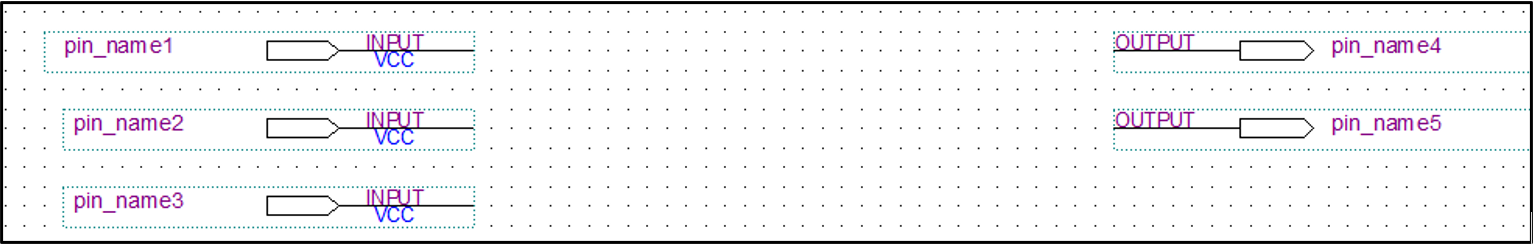
\includegraphics[width=\textwidth]{./figs/pin_names.png}
    \caption{Pinos de entrada e saída do somador completo antes da nomeação dos terminais.}
    \label{fig:pin_names}
\end{figure}

Para editar os nomes dos terminais de acordo com o projeto, utilize o sobrescrito para representar espaços quando houver. Por exemplo, um terminal nomeado como \texttt{Carry in} deve ser editado para \texttt{Carry\_in}, pois o programa não aceita espaços para o nome dos terminais. Seu esquemático deverá ficar parecido com o ilustrado na Figura~\ref{fig:pin_names_named}.

\begin{figure}[htbp!]
    \centering
    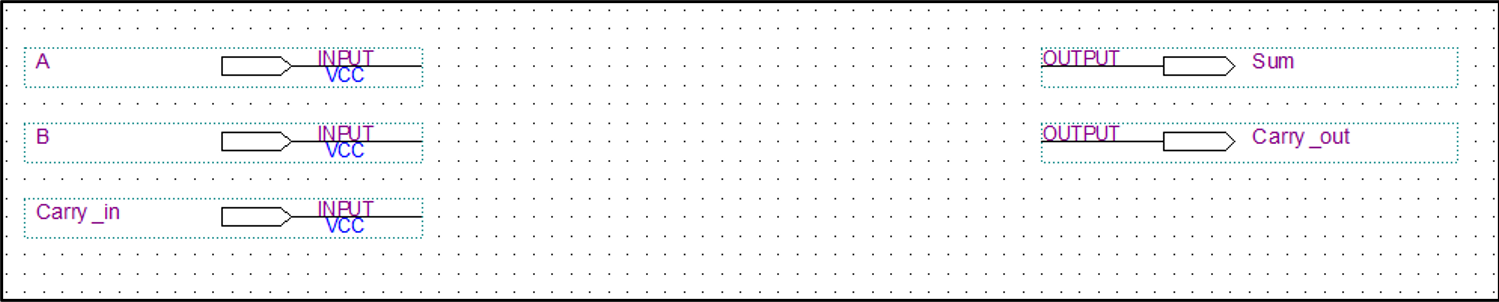
\includegraphics[width=\textwidth]{./figs/pin_names_named.png}
    \caption{Pinos de entrada e saída do somador completo antes da nomeação dos terminais.}
    \label{fig:pin_names_named}
\end{figure}

Para acrescentar as portas lógicas ou outros dispositivos básicos, clique em \textbf{Symbol tool} (\raisebox{-0.25\height}{
\includegraphics[height=12pt]{./figs/symb.png}}). Uma janela deverá ser exibida, conforme ilustrado na Figura~\ref{fig:symbol}. No campo \texttt{Libraries}, navegue, seguindo o indicado na Figura~\ref{fig:symbol}, na pasta de bibliotecas do Quartus até chegar em \texttt{logic} (subpasta de \texttt{primitives}). Esta pasta contém exclusivamente portas lógicas. 

\begin{figure}[htbp!]
    \centering
    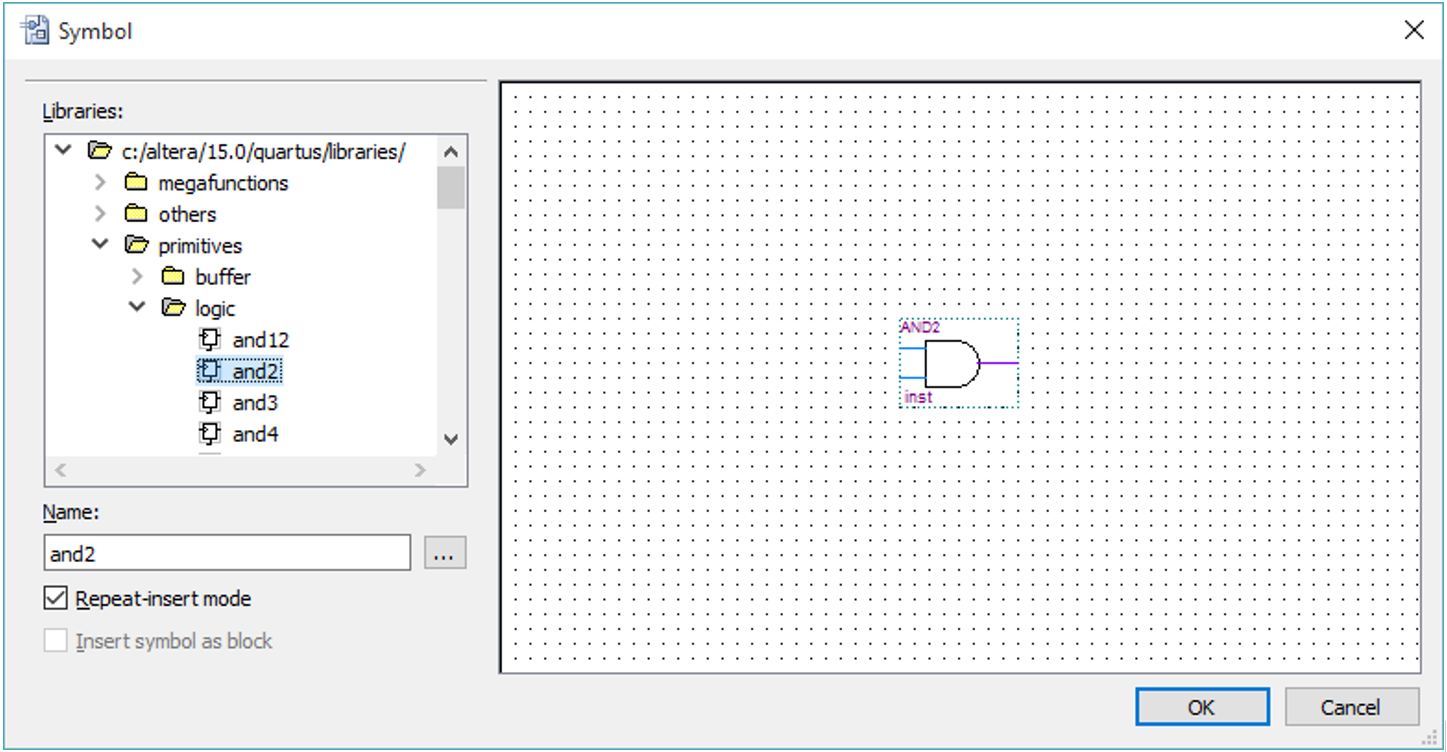
\includegraphics[width=\textwidth]{./figs/symbol.png}
    \caption{Janela para inserção de símbolos digitais (\textbf{Symbol tool}).}
    \label{fig:symbol}
\end{figure}

Alternativamente, é possível especificar o nome do dispositivo lógico diretamente no campo \texttt{Name} da Figura~\ref{fig:symbol}. O dispositivo será identificado apenas se o nome completo for inserido. Por exemplo, ao digitarmos \texttt{and2} no campo \texttt{Name}, seu símbolo aparecerá no lado direito da janela, conforme ilustrado na Figura~\ref{fig:symbol}.

Para adicionar uma porta \texttt{XOR} ao seu projeto, selecione-a e clique em \texttt{OK}. O cursor do mouse será substituído pelo símbolo de uma porta \texttt{XOR}, indicando que ela pode ser posicionada em qualquer local da área de edição de circuitos. Para inserir a porta \texttt{XOR} no esquemático, clique na região desejada. Observe que o cursor permanece como o símbolo de uma porta \texttt{XOR}, permitindo a adição de uma segunda porta com outro clique no esquemático. O desenho resultante deverá assemelhar-se à Figura~\ref{fig:xor}.

\begin{figure}[htbp!]
    \centering
    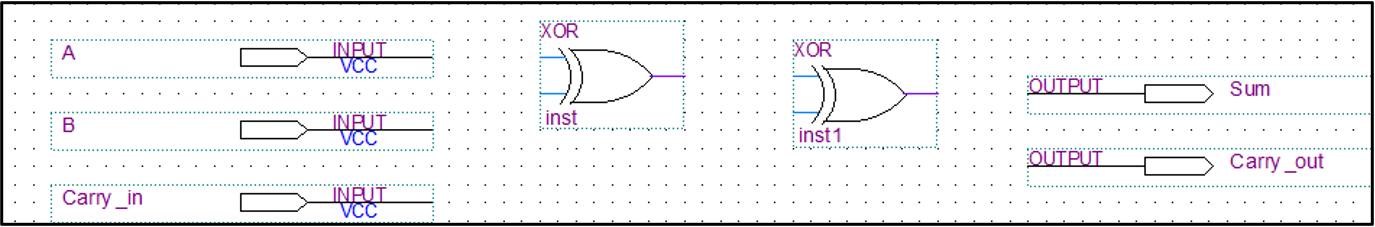
\includegraphics[width=\textwidth]{./figs/xor.png}
    \caption{Esquemático com a adição das portas \texttt{XOR}.}
    \label{fig:xor}
\end{figure}

Acrescente as outras portas necessárias para o circuito somador da mesma maneira que as portas \texttt{XOR} foram inseridas. Seu esquemático deverá assemelhar-se à Figura~\ref{fig:andxor}. Para girar um símbolo no esquemático, clique com o botão direito do mouse sobre o símbolo desejado e selecione a opção \texttt{Rotate by Degrees}. A porta \texttt{AND} de duas entradas pode ser encontrada no \textbf{Symbol Tool} como \texttt{and2}.

\begin{figure}[htbp!]
    \centering
    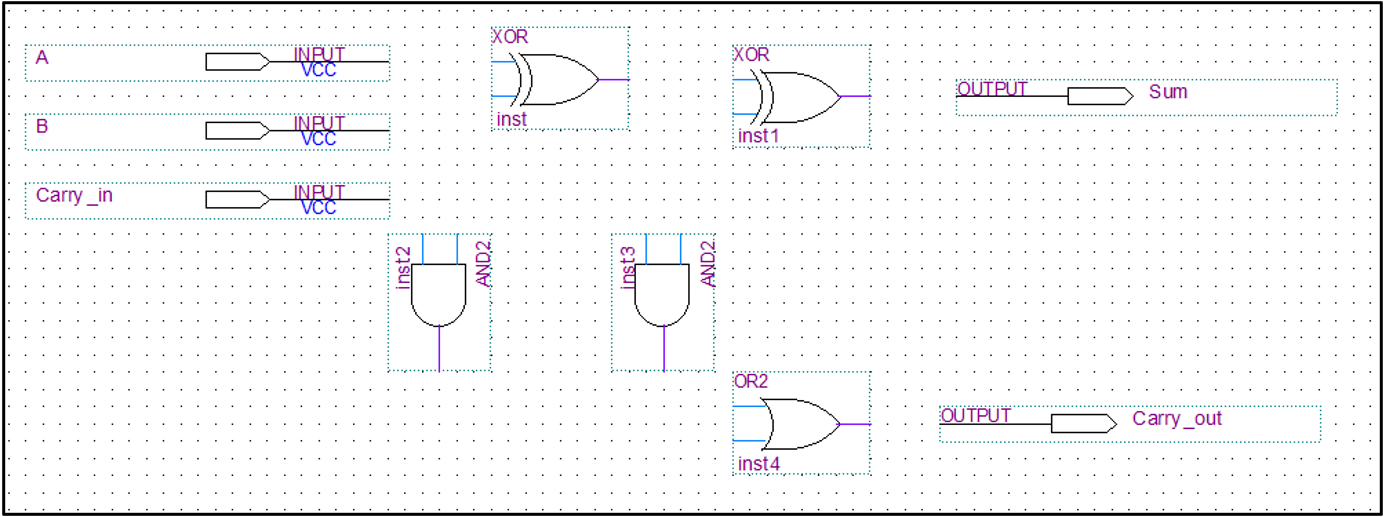
\includegraphics[width=\textwidth]{./figs/andxor.png}
    \caption{Esquemático do somador completo com todas as portas inseridas, mas sem as ligações.}
    \label{fig:andxor}
\end{figure}

Para finalizar o circuito somador completo, resta fazer as ligações entre os terminais conforme ilustrado na Figura~\ref{fig:somadorCompleto}. Para isso, aproxime o cursor do mouse à extremidade de um dos terminais e observe que o símbolo do mouse será substituído por uma ``mira''. Quando isso acontecer, clique, segure e arraste o mouse até o outro ponto de conexão. Alternativamente, clique \textbf{Orthogonal node toll} (\raisebox{-0.25\height}{
\includegraphics[height=12pt]{./figs/conect.png}}) para inserir linhas de conexão. Após realizar as ligações, seu circuito será semelhante à Figura~\ref{fig:somadorFeito}. Salve o esquemático com o nome \texttt{somador\_completo.bdf}, onde \texttt{bdf} é a extensão do arquivo (adicionada automaticamente). Não feche este esquemático.

\Attention{Certifique-se de salvar o arquivo do somador completo com o nome \texttt{somador\_completo.bdf}. Isso é importante para os próximos passos.}

\begin{figure}[htbp!]
    \centering
    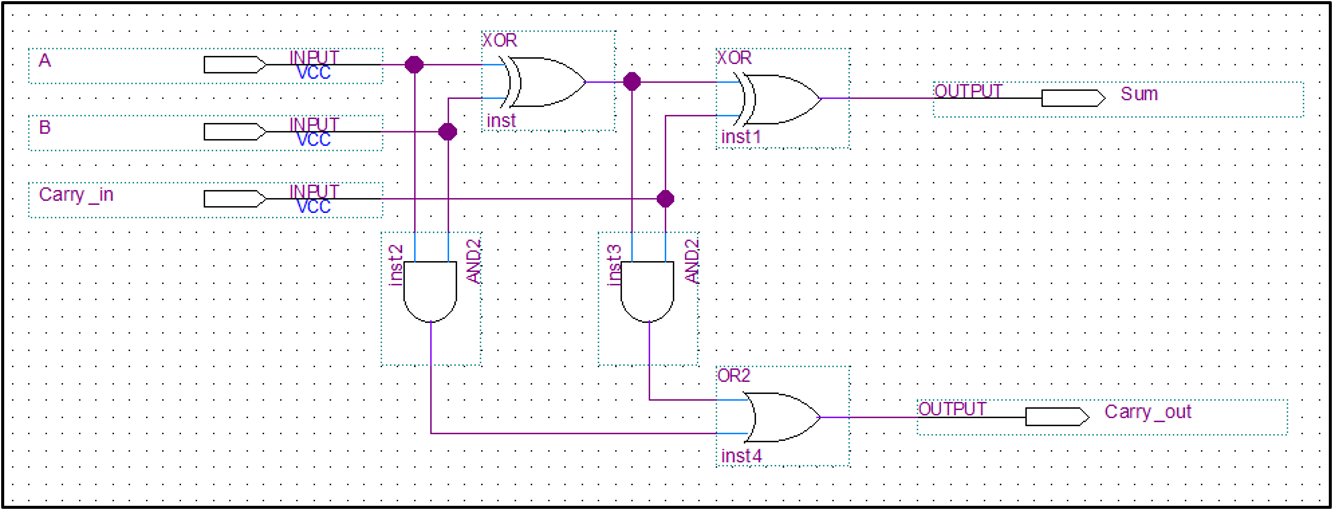
\includegraphics[width=\textwidth]{./figs/somadorFeito.png}
    \caption{Esquemático do somador completo com todas as portas inseridas, e conexões completas.}
    \label{fig:somadorFeito}
\end{figure}

\section{Criando um bloco lógico}

Para reaproveitar um circuito em diferentes esquemáticos, é necessário criar um novo bloco lógico. Este processo inclui a criação do símbolo lógico para o circuito que deseja-se reutilizar. Como exemplo, na construção de um somador \textit{carry ripple} de 4 bits, o somador completo precisa ser replicado quatro vezes e ligado em série. A Figura~\ref{fig:somadorCompletoLigado} mostra essa configuração, com as entradas X3, X2, X1, e X0 representando uma parcela da soma, e Y3, Y2, Y1, e Y0 a outra parcela. As saídas S3, S2, S1, e S0 apresentam o resultado da soma, enquanto \texttt{Cout} é o \texttt{carry} de saída, que indica se o total excede o valor representável por quatro bits (``1111''). O \texttt{carry} de entrada é mantido em nível lógico baixo.

\begin{figure}[htbp!]
    \centering
    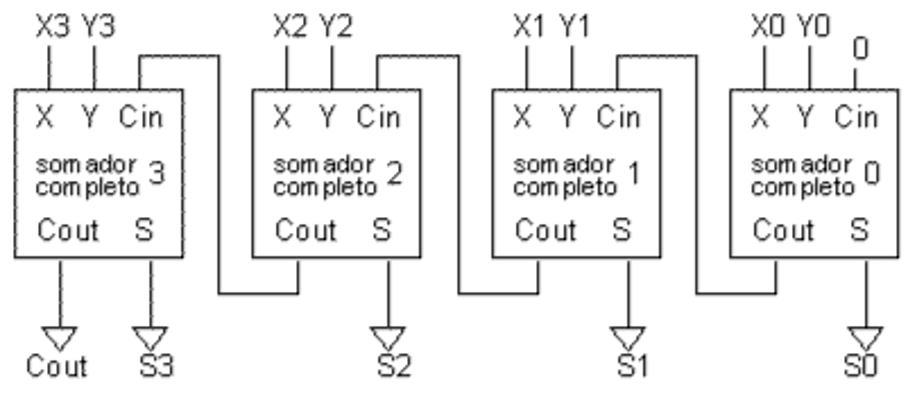
\includegraphics[width=0.6\textwidth]{./figs/somadorCompleto.png}
    \caption{Ligação em série de somadores completos para formar um somador \textit{Carry ripple} de quatro bits.}
    \label{fig:somadorCompletoLigado}
\end{figure}

Embora seja possível desenhar o circuito inteiro utilizando apenas portas lógicas, essa abordagem tornaria a visualização e compreensão do design muito complexas. Por isso, o Quartus oferece a opção de criar blocos lógicos, que simplificam o esquemático e podem ser reutilizados em diferentes projetos, facilitando tanto o design quanto a análise do circuito.

Para a criação de um \textbf{bloco somador completo}, verifique se o esquemático do circuito está aberto em primeiro plano no Quartus. Em seguida, siga os passos abaixo:

\begin{enumerate}
    \item Clique em \texttt{File} $\rightarrow$ \texttt{Create/Update} $\rightarrow$ \texttt{Create Symbol Files for Current File}.
    \item Salve o arquivo na pasta do projeto com o nome \texttt{"somador\_completo.bsf"} (sem as aspas). 
\end{enumerate}

A extensão \texttt{.bsf} indica que o arquivo é um \textit{bloco lógico} (\textit{block symbol file}) que pode ser utilizado em outros esquemáticos.

\Attention{Tenha certeza de salvar o esquemático do somador completo com o nome \texttt{"somador\_completo.bsf"} (sem as aspas). Isso é importante para a sequência desse tutorial.}

\section{Reaproveitando o bloco criado}

O \textbf{top level design} é o arquivo principal do projeto e deve conter o circuito \textit{somador de 4 bits} ilustrado na Figura 15. Para criar um novo arquivo esquemático, siga os passos abaixo:

\begin{enumerate}
    \item Clique em \texttt{File} $\rightarrow$ \texttt{New} e escolha \texttt{Block Diagram/Schematic File}.
\end{enumerate}

A seguir, vamos acrescentar as entradas e saídas ao esquemático. É interessante notar que algumas entradas podem ser representadas como um \textit{array de bits}, a exemplo das parcelas e do resultado da soma. Proceda da seguinte forma para adicionar as entradas e saídas:

\begin{itemize}
    \item Acrescente três entradas e duas saídas ao esquemático.
    \item Nomeie a entrada \texttt{X} como \texttt{X[3..0]}. Ao fazer isso, estamos indicando ao programa que esse terminal é formado por quatro pinos, onde o bit mais significativo (MSB) é \texttt{X[3]} e o bit menos significativo (LSB) é \texttt{X[0]}. Ou seja, o índice ou intervalo de índices do terminal deve ser informado dentro dos colchetes que seguem o nome do terminal.
    \item Repita o processo para a entrada \texttt{Y} e para a saída \texttt{S}.
    \item Nomeie a terceira entrada como \texttt{Cin} e a última saída como \texttt{Cout}.
\end{itemize}

O esquemático resultante deverá ser semelhante à Figura~\ref{fig:carryRipplePins}.

\begin{figure}[htbp!]
    \centering
    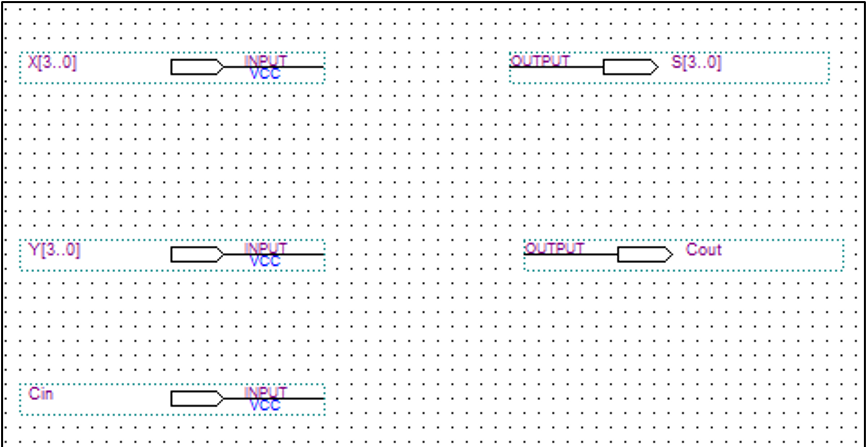
\includegraphics[width=\textwidth]{./figs/carryRipplePins.png}
    \caption{Entradas es saídas do somador \textit{Carry Ripple}.}
    \label{fig:carryRipplePins}
\end{figure}

Para inserir os \textbf{blocos dos somadores completos}, selecione a ferramenta \textbf{Symbol tool} (\raisebox{-0.25\height}{
\includegraphics[height=12pt]{figs/symb.png}}), procedendo da mesma forma empregada na elaboração do esquemático do somador completo. A ação subsequente desencadeará a exibição da janela de seleção de dispositivos, conforme ilustrado na Figura~\ref{fig:symbolSomador}.

\begin{figure}[htbp!]
    \centering
    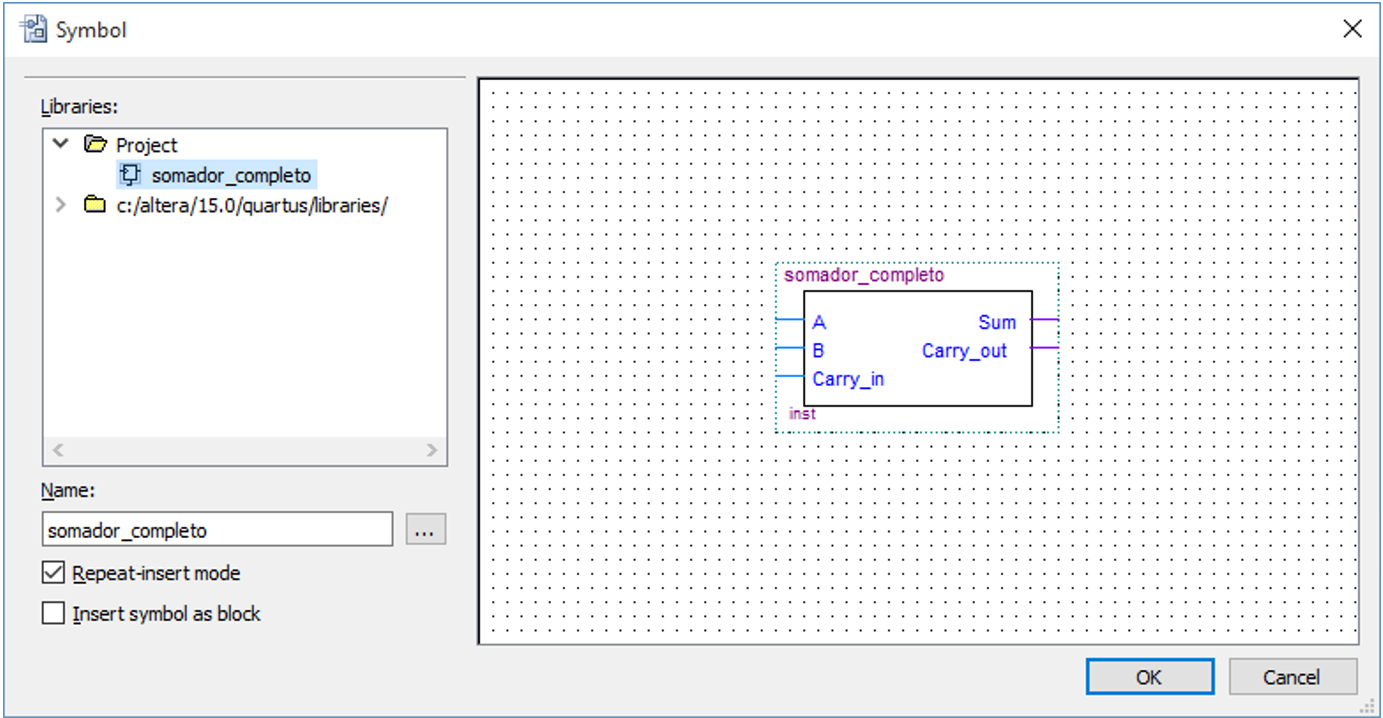
\includegraphics[width=\textwidth]{./figs/symbolSomador.png}
    \caption{\textbf{Symbol tool} com o somador completo disponível.}
    \label{fig:symbolSomador}
\end{figure}

Nesta etapa, observa-se a disponibilização de uma nova pasta no campo \texttt{Lybraries}, denominada ``\texttt{Project}'', que incorpora todos os blocos desenvolvidos ao longo do projeto. Nota-se que o único componente disponível é o \texttt{somador\_completo}. Proceda com a inserção de quatro instancias do somador completo no esquemático, conforme demonstrado na Figura~\ref{fig:18}.

\begin{figure}[htbp!]
    \centering
    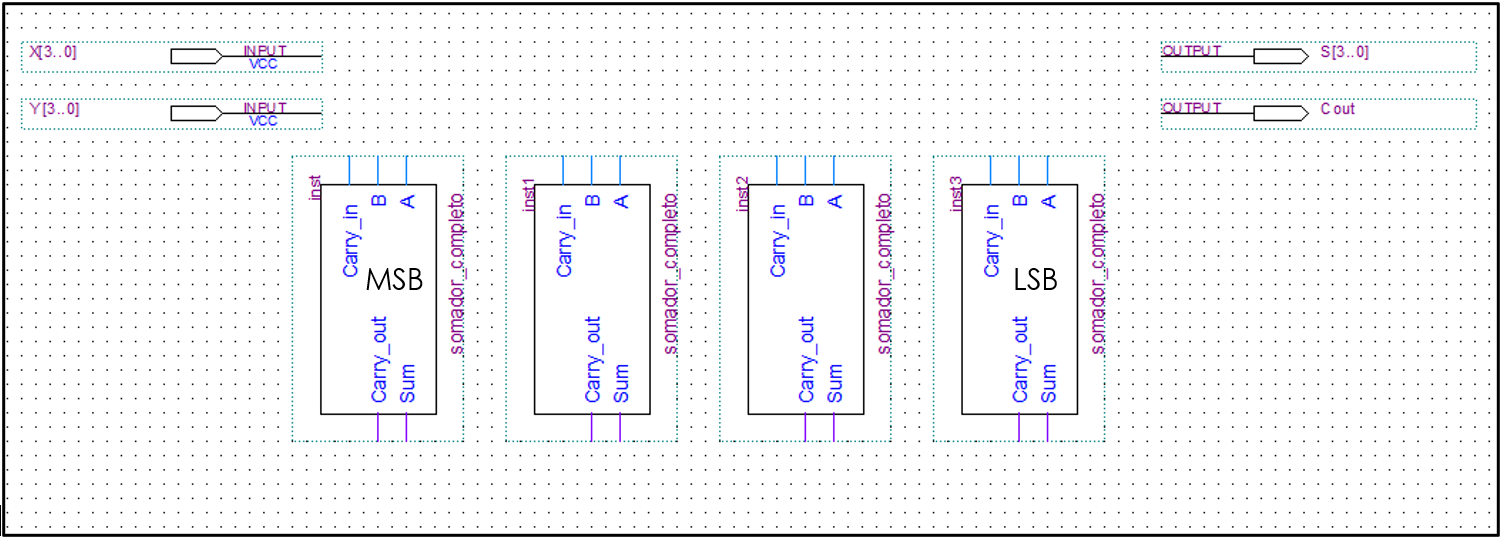
\includegraphics[width=\textwidth]{./figs/fig18.png}
    \caption{Posicionamento de quatro instancias do \texttt{somador\_completo}.}
    \label{fig:18}
\end{figure}

Neste exemplo, optamos por designar que o bloco mais à direita somará os LSBs de \texttt{X} e \texttt{Y}, gerando o LSB da soma. As entradas \texttt{X} e \texttt{Y} são conjuntos de bits (4 bits cada um), e ao tentar desenhar uma linha partindo de uma dessas entradas, notamos a formação de uma linha mais espessa, indicando que se trata de um barramento de bits (para o caso em análise, um barramento de 4 bits). Portanto, é necessário derivar os bits correspondentes para conectá-los às entradas apropriadas nos somadores completos. Para isso, trace um barramento saindo do terminal de \texttt{X} até que este barramento abranja todos os somadores, conforme ilustrado na Figura \ref{fig:19}.

\begin{figure}[htbp!]
    \centering
    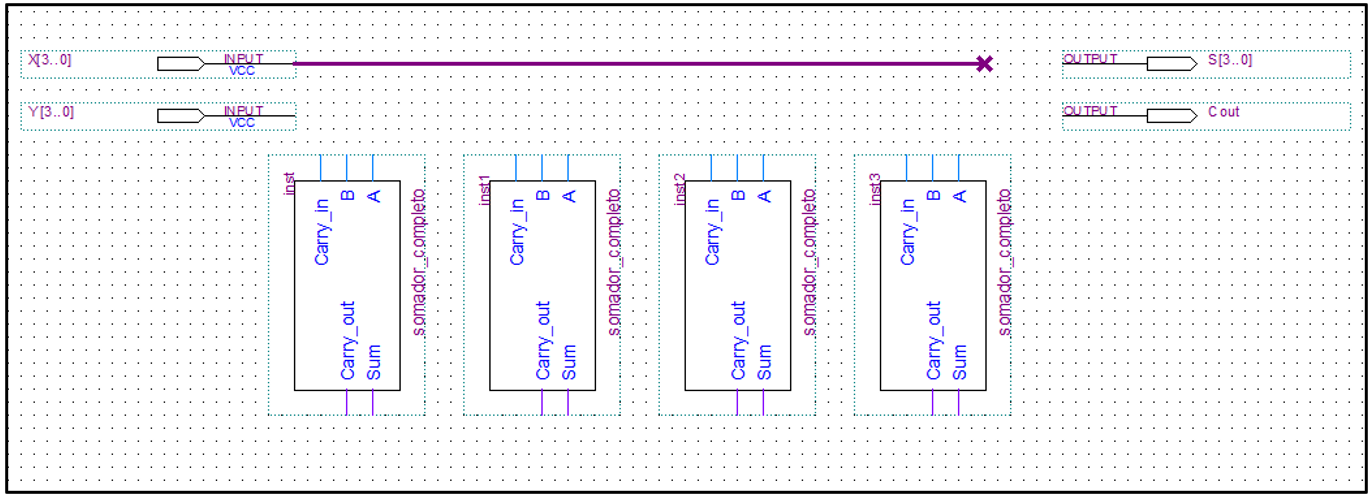
\includegraphics[width=\textwidth]{./figs/fig19.png}
    \caption{Traçando um barramento a partir da entrada \texttt{X} que possui 4 bits.}
    \label{fig:19}
\end{figure}

Em seguida, conecte as entradas \texttt{A} de cada \texttt{somador\_completo} ao barramento. Para isso, posicione o mouse no terminal \texttt{A} e, ao visualizar o símbolo do alvo, clique, segure e arraste-o até o barramento. Após realizar a conexão nas quatro instancias, clique com o botão direito do mouse sobre o fio do LSB e selecione ``\texttt{properties}''. No campo \texttt{name} da aba \texttt{general}, digite: \texttt{X[0]}, e clique em \texttt{OK}. Esta ação designa que a conexão corresponde ao bit menos significativo de \texttt{X}. Repita o procedimento para as outras três conexões, e o esquemático apresentará semelhanças com a Figura~\ref{fig:20}. Execute o mesmo processo para a entrada \texttt{Y} e para a saída \texttt{S}, conforme ilustrado na Figura 21.

\begin{figure}[htbp!]
    \centering
    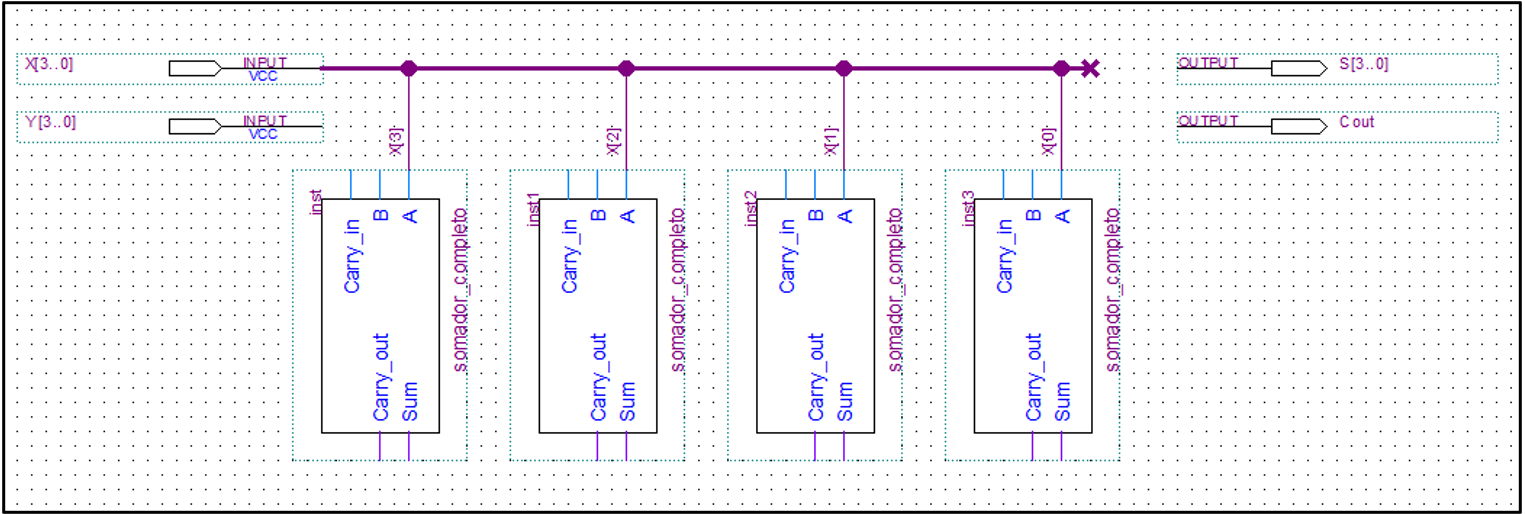
\includegraphics[width=\textwidth]{./figs/fig20.png}
    \caption{Ligando o barramento \texttt{X} às respectivas entradas das instancias do \texttt{somador\_completo}.}
    \label{fig:20}
\end{figure}

\begin{figure}[htbp!]
    \centering
    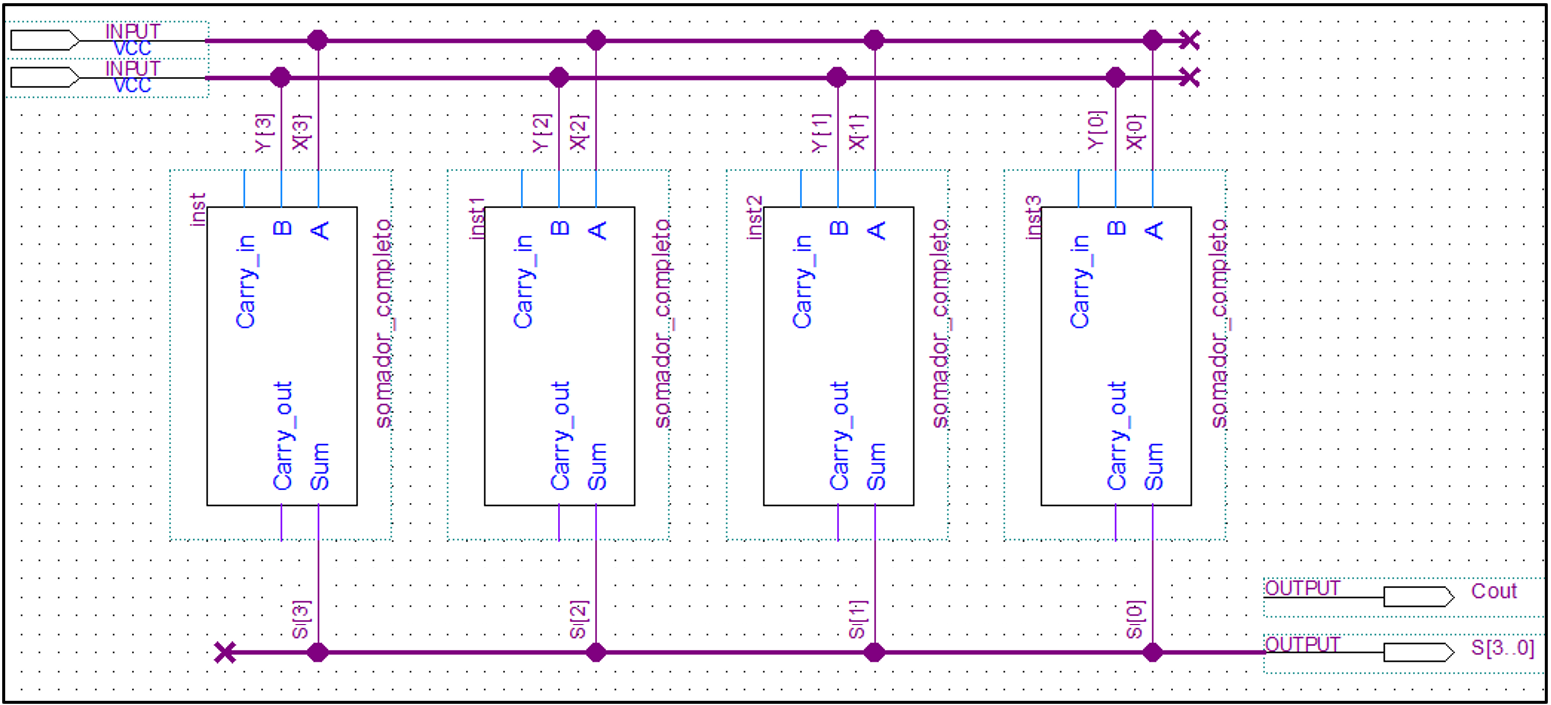
\includegraphics[width=\textwidth]{./figs/fig21.png}
    \caption{Ligando os barramentos \texttt{X}, \texttt{Y} e \texttt{S} às respectivas entradas e saídas das instancias do \texttt{somador\_completo}.}
    \label{fig:21}
\end{figure}

\begin{figure}[htbp!]
    \centering
    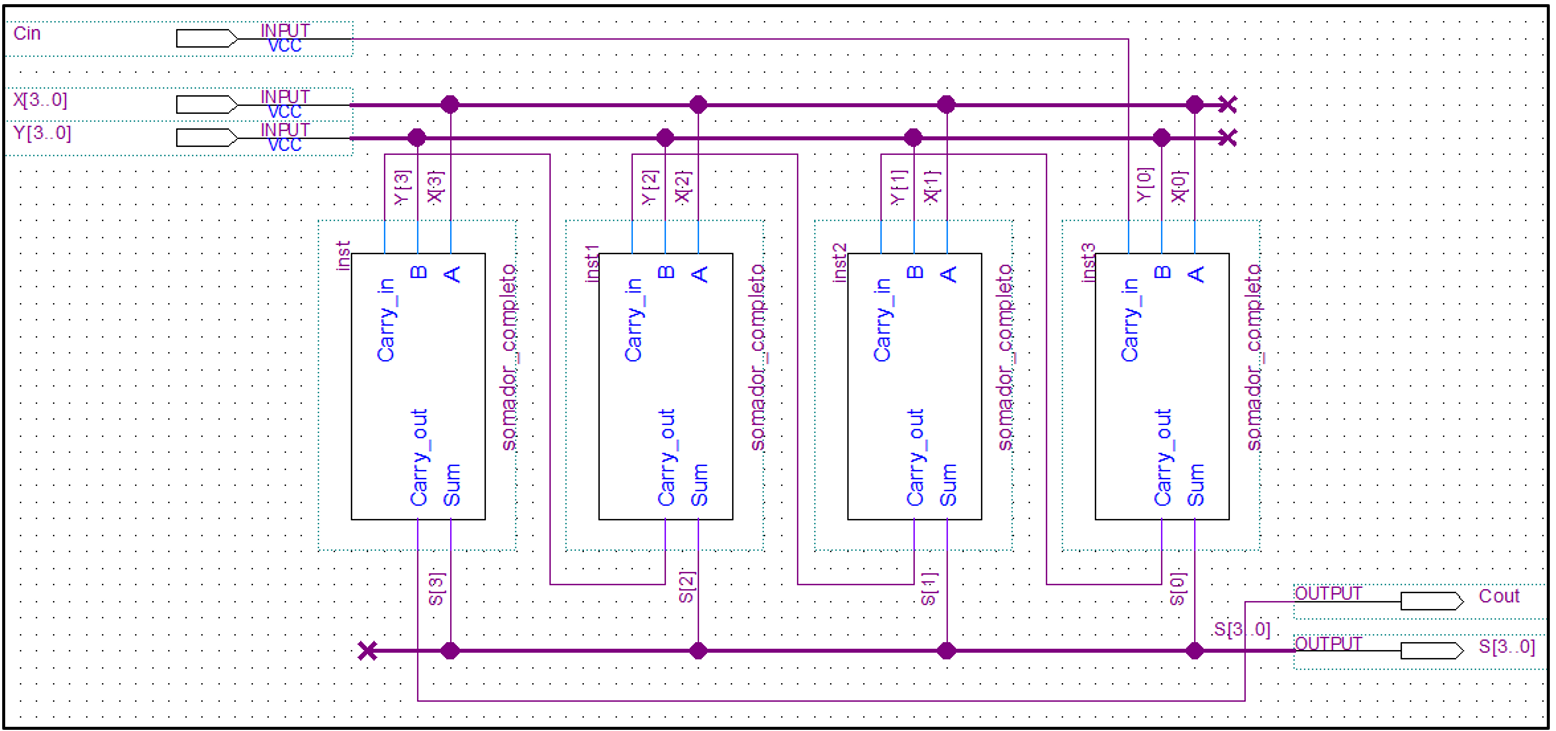
\includegraphics[width=\textwidth]{./figs/fig22.png}
    \caption{Esquemático do \texttt{somador\_de\_4\_bits} finalizado.}
    \label{fig:22}
\end{figure}

Complete o esquemático conforme indicado na Figura~\ref{fig:22}. Observe que uma nova entrada denominada \texttt{Cin} foi vinculada ao carry de entrada do somador que processa os LSBs. Salve o diagrama com o nome \texttt{somador\_de\_4\_bits.bdf}, que corresponde ao nome do design de nível superior (\textit{top-level design}) estabelecido no início do projeto. Se o esquemático for salvo com um nome diferente, ocorrerão erros durante a análise do projeto.

\Attention{Salve o diagrama com o nome \texttt{somador\_de\_4\_bits.bdf}, que corresponde ao nome do design de nível superior (\textit{top-level design}) estabelecido no início do projeto. Se o esquemático for salvo com um nome diferente, ocorrerão erros durante a análise do projeto.}

\section{Análise e Síntese}

A compilação de um projeto no Quartus ou em qualquer outra IDE para PLDs envolve vários passos. No caso do Quartus a primeira etapa é chamada de \textit{Analysis and Synthesis} (Análise e Síntese). As diversas etapas podem ser observadas no quadro \texttt{Tasks} que geralmente fica no canto esquerdo da tela, conforme a Figura~\ref{fig:23}. Para o intuito deste tutorial exploraremos apenas essa primeira etapa.

\begin{figure}[htbp!]
    \centering
    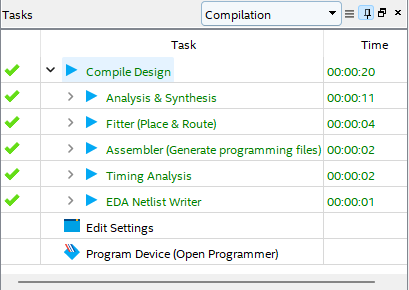
\includegraphics[width=0.4\textwidth]{./figs/fig23.png}
    \caption{Quadro \texttt{Tasks} do quartus mostrando as etapas de compilação.}
    \label{fig:23}
\end{figure}

A análise e síntese no Quartus, representam etapas fundamentais no processo de desenvolvimento de circuitos digitais, especialmente para FPGAs (\textit{Field Programmable Gate Arrays}) e CPLDs (\textit{Complex Programmable Logic Devices}).

Durante a etapa de \textbf{análise}, o Quartus examina o código ou o esquemático submetido para o projeto, que pode estar em VHDL, Verilog, ou como um esquemático gráfico. Esta fase inclui a verificação da sintaxe e da semântica do código ou do esquemático, garantindo que eles estejam isentos de erros e sejam interpretáveis pela ferramenta. A análise assegura a correção do design em relação às regras da linguagem de descrição de hardware utilizada e às especificações do projeto.

Após a análise, ocorre a \textbf{síntese}, que é o processo de conversão do código ou esquemático de alto nível em uma representação de baixo nível que mapeia diretamente para os recursos físicos do dispositivo alvo, como lógica programável, células lógicas, blocos de memória, entre outros. Durante a síntese, a ferramenta realiza otimizações no design para melhorar o desempenho e a utilização dos recursos, respeitando as restrições definidas pelo usuário (tais como frequência de operação, consumo de energia, tamanho, etc.).

O resultado da síntese é um \textit{netlist}, que pode ser traduzido como ``lista de interconexões'', descrevendo como os blocos lógicos são interconectados dentro do FPGA ou CPLD. Esse \textit{netlist} é então utilizado nas etapas subsequentes do processo de design, como a colocação e o roteamento (\textit{place and route} ou \textit{fitter}), onde a ferramenta determina a localização física dos componentes no dispositivo e como eles serão interconectados fisicamente. O \textit{netlist} também pode ser utilizado para a realização de simulações.

Com o esquemático finalizado, a próxima etapa é proceder com a análise e síntese do circuito, permitindo que o programa execute simulações funcionais. O processo de análise tem por objetivo verificar a presença de erros ou incoerências no projeto. Para iniciar a análise e a síntese, pressione \texttt{Ctrl + K}, ou clique no botão correspondente na parte superior da janela do Quartus (\raisebox{-0.25\height}{
\includegraphics[height=12pt]{figs/bt_as.png}}) ou dê um duplo clique sobre \texttt{Analysis \& Synthesis} no quadro \texttt{Tasks}. Aguarde alguns minutos para que o processo seja concluído. Caso sejam identificados erros, efetue as correções necessárias e repita o procedimento.

\section{Simulação funcional}

A \textbf{simulação funcional} é um tipo de simulação utilizada no design de circuitos eletrônicos, especialmente em circuitos digitais e sistemas embarcados, para verificar o comportamento lógico do design. Ela é realizada antes ou durante as fases iniciais do processo de desenvolvimento para garantir que o circuito ou sistema realiza as funções desejadas conforme especificado, sem considerar os aspectos físicos como tempos de atraso, capacidade de carga, ou outras características elétricas do hardware.

No Quartus, clique em \texttt{File $\rightarrow$ New} e escolha a opção \texttt{University Program VWF}. Uma nova janela se abrirá, conforme a Figura~\ref{fig:24}. Observe que o arquivo está vazio e sem possibilidade de configuração; para adicionar os terminais que serão simulados (entradas e saídas do circuito somador de 4 bits), clique em \texttt{Edit $\rightarrow$ Insert $\rightarrow$ Insert Node or Bus...} e uma nova janela se abrirá, conforme ilustrado na Figura~\ref{fig:25}. Nesta nova janela, clique no botão \texttt{Node Finder}, que abrirá a janela da Figura~\ref{fig:26}

\begin{figure}[htbp!]
    \centering
    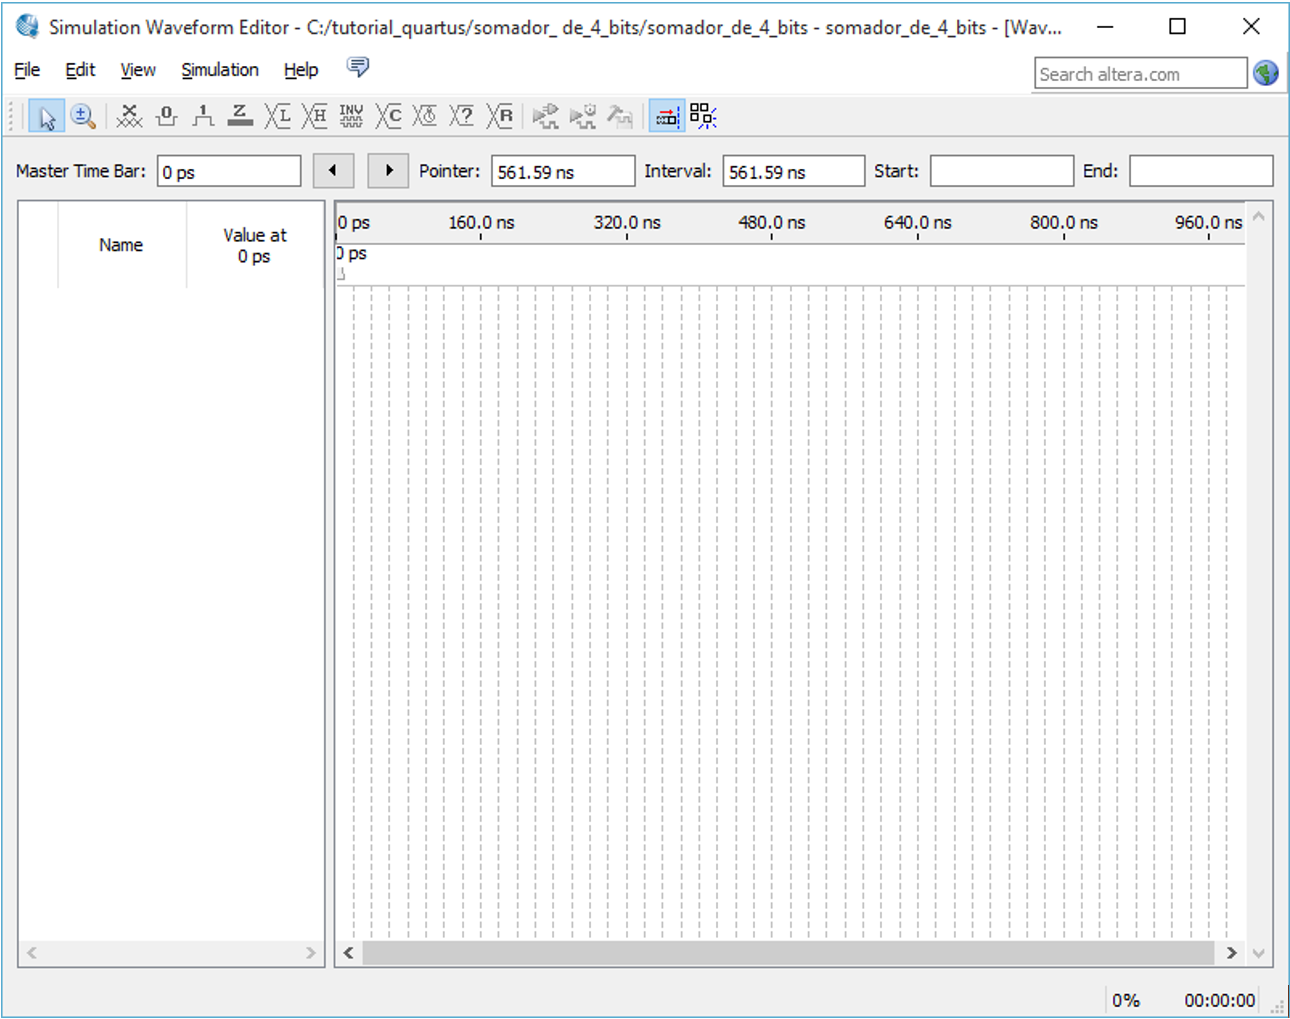
\includegraphics[width=\textwidth]{./figs/fig24.png}
    \caption{Ambiente de simulação do \texttt{University Program VWF}.}
    \label{fig:24}
\end{figure}

\begin{figure}[htbp!]
    \centering
    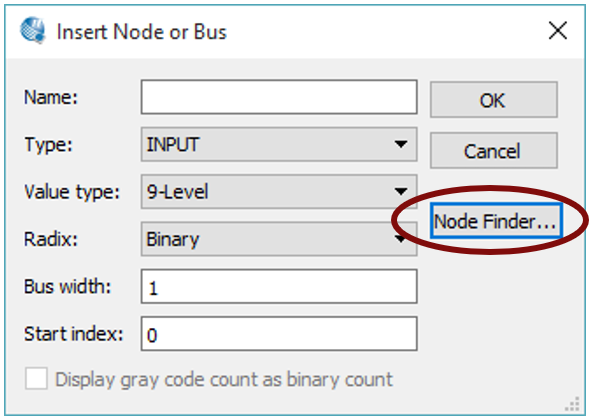
\includegraphics[width=0.6\textwidth]{./figs/fig25.png}
    \caption{Janela \texttt{Insert node or bus}.}
    \label{fig:25}
\end{figure}

\begin{figure}[htbp!]
    \centering
    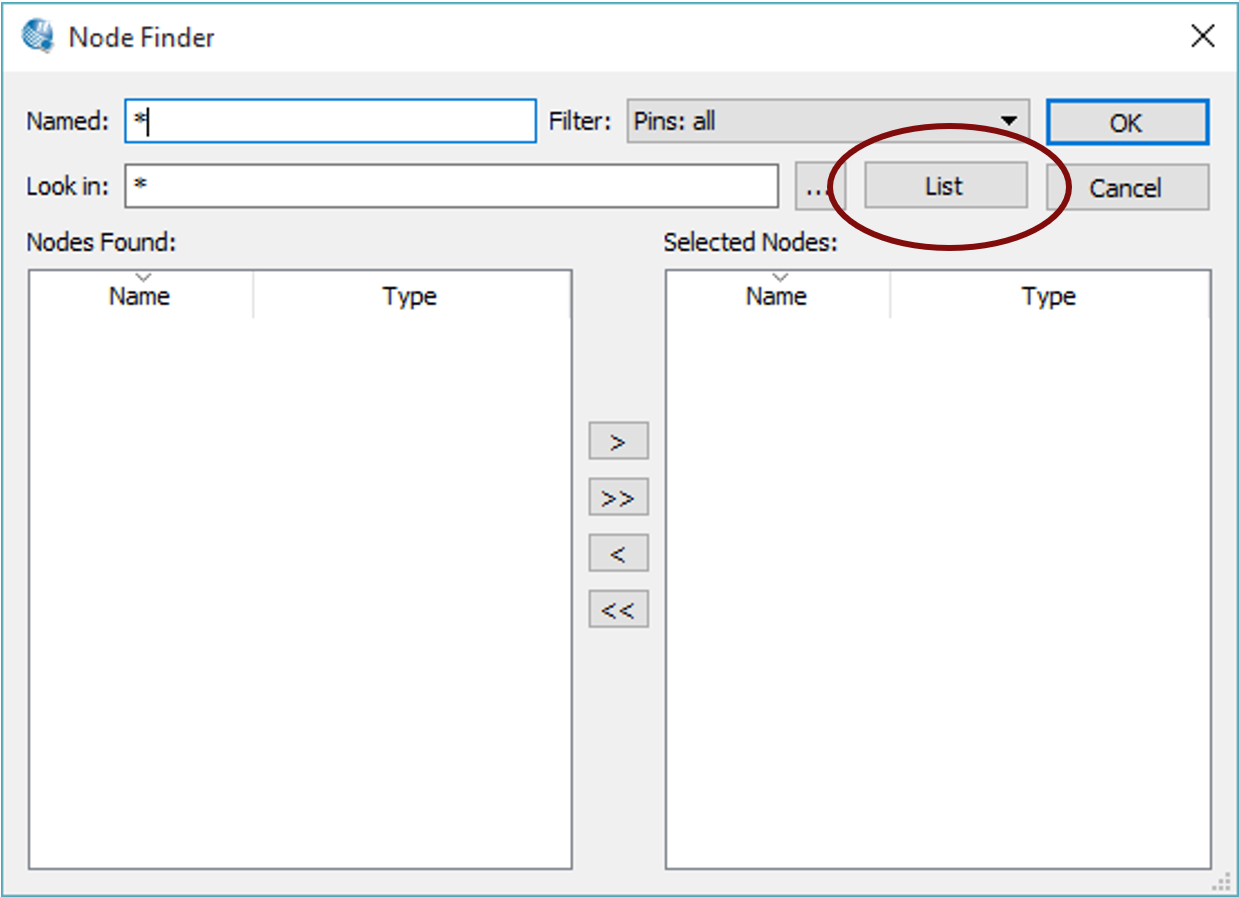
\includegraphics[width=0.6\textwidth]{./figs/fig26.png}
    \caption{Janela \texttt{Node finder}.}
    \label{fig:26}
\end{figure}

Clique em \texttt{List} e os terminais de entrada e saída do projeto serão exibidos no campo \texttt{Nodes Found}. Clique no botão com o símbolo ``\texttt{>>}'' para selecionar todos os terminais criados no projeto. Clique em \texttt{OK} e, novamente, em \texttt{OK}. O ambiente de simulação ficará similar ao apresentado na Figura~\ref{fig:27}.

\begin{figure}[htbp!]
    \centering
    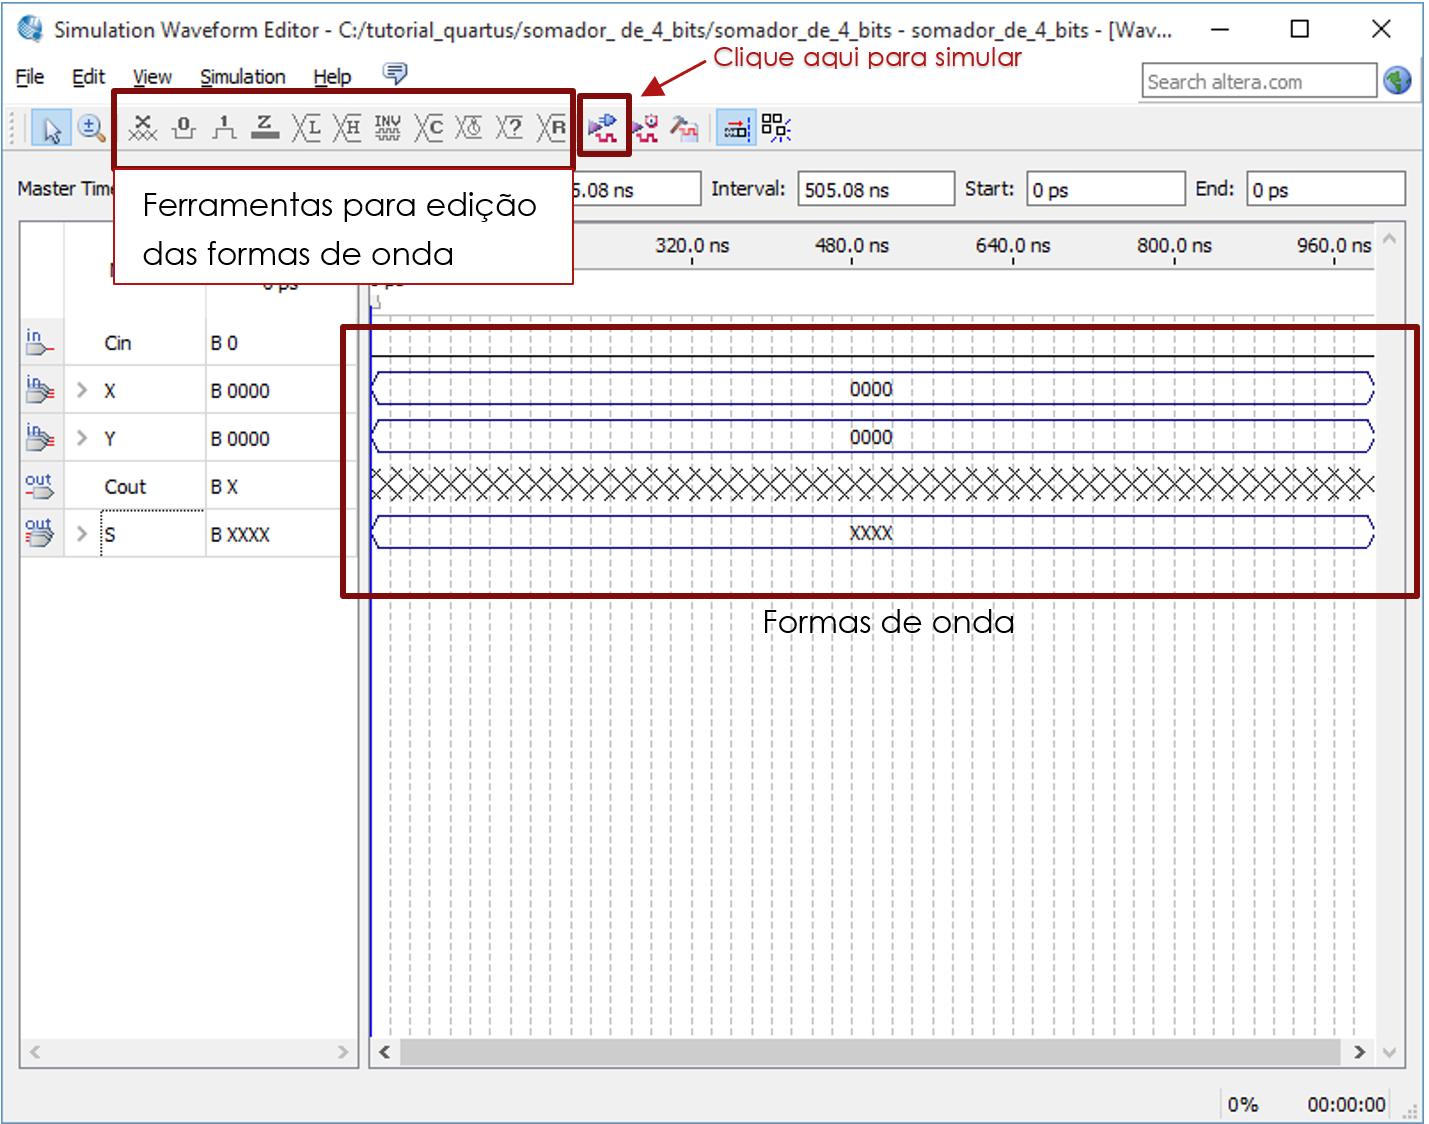
\includegraphics[width=\textwidth]{./figs/fig27.png}
    \caption{Ambiente de simulação do \texttt{University Program VWF} com as entradas e saídas inseridas e prontas para edição.}
    \label{fig:27}
\end{figure}

No canto direito do ambiente de simulação, conforme visto na Figura~\ref{fig:27}, encontram-se as formas de onda que podem ser editadas. É importante enfatizar que somente as formas de onda de terminais classificados como de entrada e bidirecionais estão sujeitas à edição. As ferramentas para edição das formas de onda digitais localizam-se no canto superior esquerdo. 

A manipulação das formas de onda de entrada é intuitiva. Para editar, selecione com o mouse (clicando e arrastando) a faixa de tempo desejada em um dos terminais de entrada e empregue uma das ferramentas disponíveis para modificar os valores lógicos dos sinais. Por exemplo, caso seja necessário inserir o valor binário ``1100'' em \texttt{X}, no intervalo de tempo de 0 a 300 ns, deve-se selecionar o intervalo de tempo correspondente para a entrada \texttt{X}. Após a seleção, clica-se no botão com o símbolo de interrogação para forçar a entrada de um valor arbitrário. Consequentemente, uma janela será aberta permitindo a inserção do valor desejado.

Proceda com a edição das formas de onda de \texttt{X}, \texttt{Y}, e \texttt{Cin} de maneira a testar exaustivamente o circuito. Confira se a operação de soma está sendo executada corretamente. Este momento também é oportuno para explorar as funcionalidades de cada ferramenta de edição. Para iniciar a simulação, clique no botão indicado na Figura~\ref{fig:27} (\texttt{Run Functional Simulation}), é possível que seja solicitado que o arquivo de simulação seja salvo.

A Figura 28 ilustra o resultado de uma simulação para o circuito somador de 4 bits. Importante ressaltar que a simulação funcional considera apenas o uso de componentes ideais, desconsiderando, portanto, quaisquer tempos de atraso. Uma simulação que incorpora a análise de tempos de atraso é denominada simulação temporal e será abordada em outro tutorial.

\begin{figure}[htbp!]
    \centering
    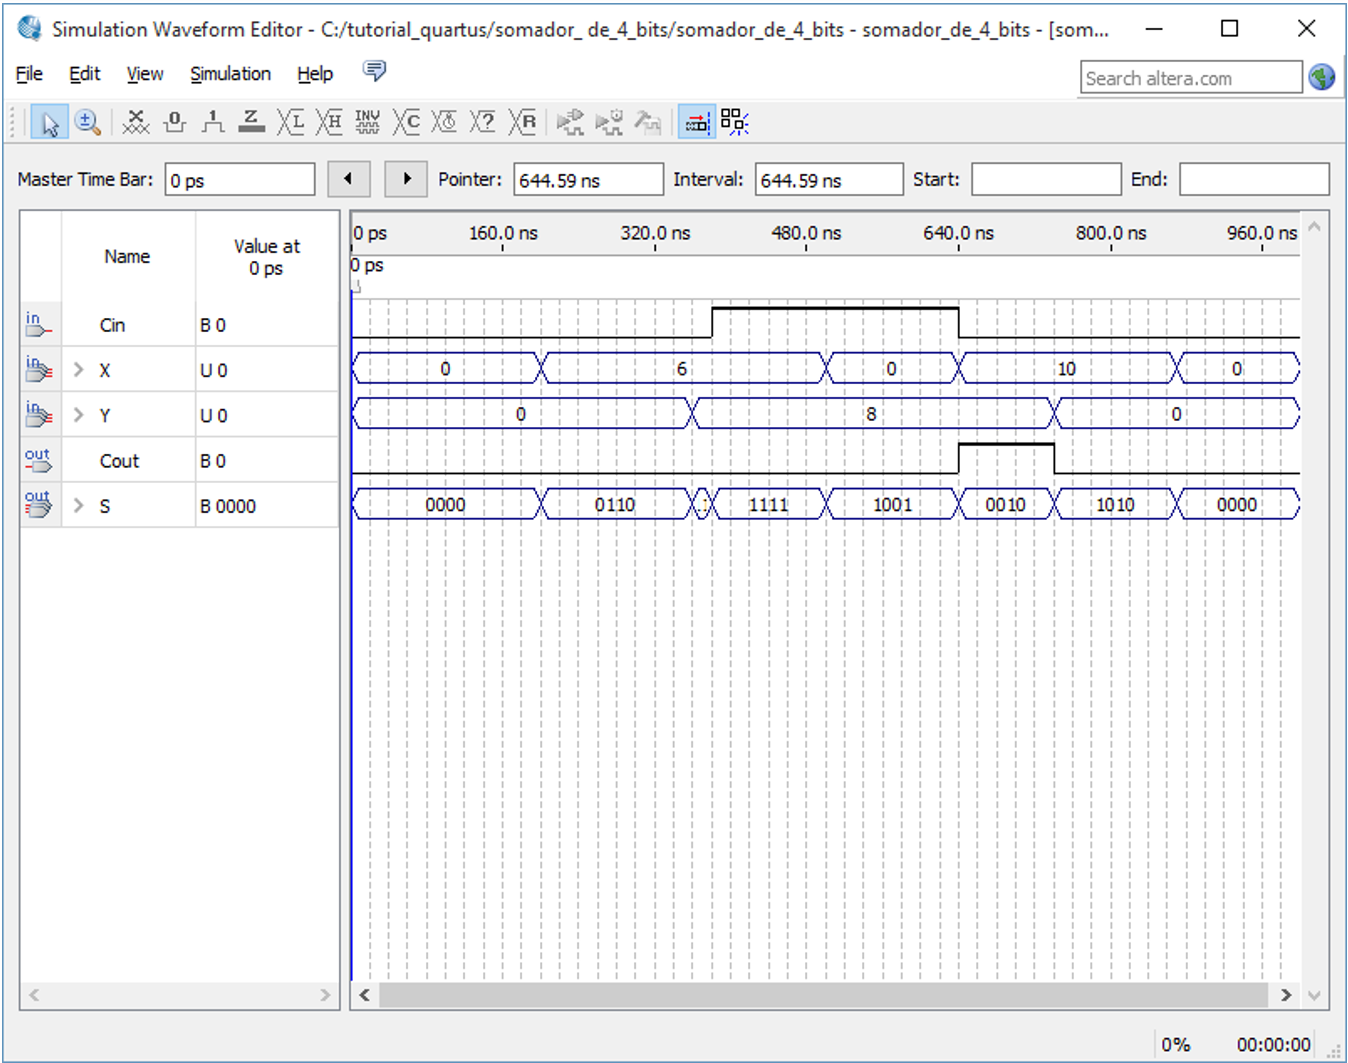
\includegraphics[width=\textwidth]{./figs/fig28.png}
    \caption{Exemplo de resultado de simulação para o somador de 4 bits.}
    \label{fig:28}
\end{figure}

\newpage
\bibliographystyle{IEEEtran} % Define o estilo das referências. Opções comuns: plain, unsrt, alpha, abbrv.
\bibliography{refs} % O nome do arquivo .bib (sem a extensão).




\end{document}
